\section{CaloChallenge 2022}
{{\footnotesize
\begin{description}[labelwidth=5em, labelsep=1em, leftmargin=*, align=left, itemsep=0.3em, parsep=0em]
  \item[date:] 2024-10-28
  \item[last\_updated:] 2024-10
  \item[expired:] unkown
  \item[valid:] yes
  \item[url:] \href{http://arxiv.org/abs/2410.21611}{http://arxiv.org/abs/2410.21611}
  \item[domain:] LHC Calorimeter; Particle Physics
  \item[focus:] Fast generative-model-based calorimeter shower simulation evaluation
  \item[keywords:]
    - calorimeter simulation
    - generative models
    - surrogate modeling
    - LHC
    - fast simulation
  \item[task\_types:]
    - Surrogate modeling
  \item[ai\_capability\_measured:]
    - Simulation fidelity
    - speed
    - efficiency
  \item[metrics:]
    - Histogram similarity
    - Classifier AUC
    - Generation latency
  \item[models:]
    - VAE variants
    - GAN variants
    - Normalizing flows
    - Diffusion models
  \item[ml\_motif:]
    - Surrogate
  \item[type:] Dataset
  \item[ml\_task:] Surrogate Modeling
  \item[notes:] The most comprehensive survey to date on ML-based calorimeter simulation; 31 submissions over different dataset sizes.
  \item[contact.name:] Claudius Krause (CaloChallenge Lead)
  \item[contact.email:] unkown
  \item[dataset.name:] Four LHC calorimeter shower datasets
  \item[dataset.url:] \href{various voxel resolutions}{various voxel resolutions}
  \item[results.name:] ChatGPT LLM
  \item[results.url:] \href{unkown}{unkown}
  \item[fair.reproducible:] Yes
  \item[fair.benchmark\_ready:] Yes
  \item[ratings.software.rating:] 0
  \item[ratings.software.reason:] Not analyzed.
  \item[ratings.specification.rating:] 9.0
  \item[ratings.specification.reason:] Task is clearly defined: real-time anomaly detection from high-rate LHC collisions. Latency and bandwidth constraints are mentioned, though not numerically enforced.
  \item[ratings.dataset.rating:] 9.0
  \item[ratings.dataset.reason:] Publicly available via Zenodo, with structured signal/background splits, and rich metadata; nearly fully FAIR.
  \item[ratings.metrics.rating:] 9.0
  \item[ratings.metrics.reason:] ROC-AUC and detection efficiency are clearly defined and appropriate for unsupervised anomaly detection.
  \item[ratings.reference\_solution.rating:] 8.0
  \item[ratings.reference\_solution.reason:] Several baseline methods (autoencoder, VAE, isolation forest) are evaluated; runnable versions available via community repos but not tightly bundled.
  \item[ratings.documentation.rating:] 8.0
  \item[ratings.documentation.reason:] Paper and data documentation are clear, and the dataset is widely reused. Setup requires some manual effort to reproduce full pipelines.
  \item[id:] calochallenge\_
  \item[Citations:] \cite{krause2024calochallenge2022communitychallenge}
  \item[Ratings:]
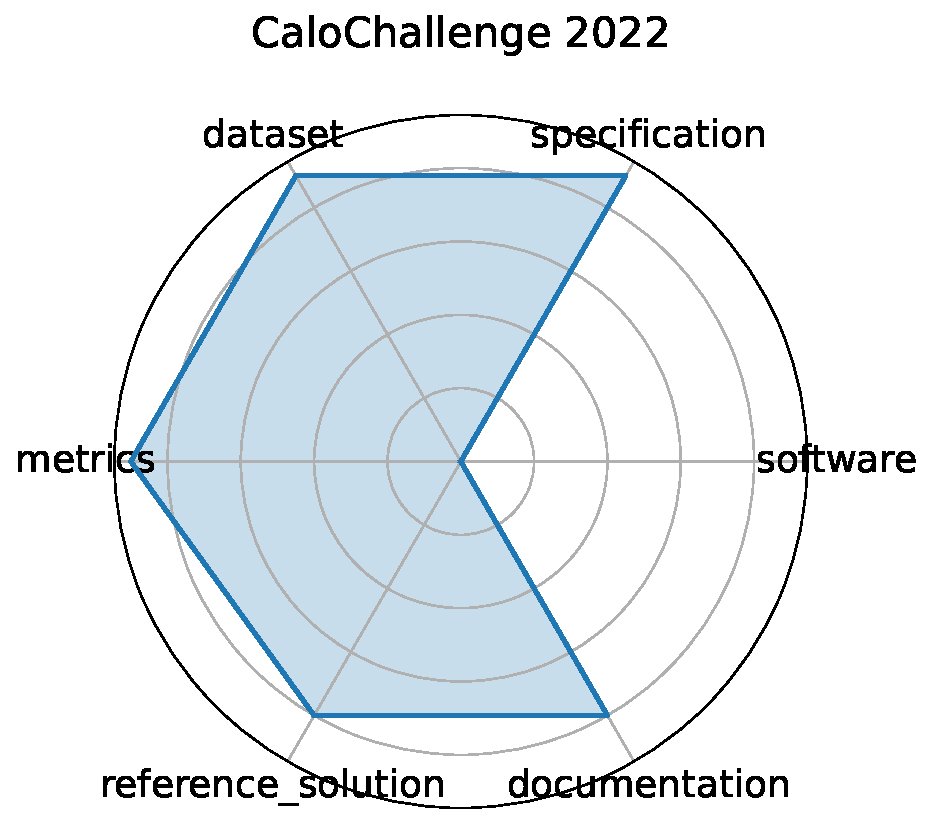
\includegraphics[width=0.2\textwidth]{calochallenge__radar.pdf}
\end{description}
}}
\clearpage